% This is "sig-alternate.tex" V2.0 May 2012
% This file should be compiled with V2.5 of "sig-alternate.cls" May 2012
%
% This example file demonstrates the use of the 'sig-alternate.cls'
% V2.5 LaTeX2e document class file. It is for those submitting
% articles to ACM Conference Proceedings WHO DO NOT WISH TO
% STRICTLY ADHERE TO THE SIGS (PUBS-BOARD-ENDORSED) STYLE.
% The 'sig-alternate.cls' file will produce a similar-looking,
% albeit, 'tighter' paper resulting in, invariably, fewer pages.
%
% ----------------------------------------------------------------------------------------------------------------
% This .tex file (and associated .cls V2.5) produces:
%       1) The Permission Statement
%       2) The Conference (location) Info information
%       3) The Copyright Line with ACM data
%       4) NO page numbers
%
% as against the acm_proc_article-sp.cls file which
% DOES NOT produce 1) thru' 3) above.
%
% Using 'sig-alternate.cls' you have control, however, from within
% the source .tex file, over both the CopyrightYear
% (defaulted to 200X) and the ACM Copyright Data
% (defaulted to X-XXXXX-XX-X/XX/XX).
% e.g.
% \CopyrightYear{2007} will cause 2007 to appear in the copyright line.
% \crdata{0-12345-67-8/90/12} will cause 0-12345-67-8/90/12 to appear in the copyright line.
%
% ---------------------------------------------------------------------------------------------------------------
% This .tex source is an example which *does* use
% the .bib file (from which the .bbl file % is produced).
% REMEMBER HOWEVER: After having produced the .bbl file,
% and prior to final submission, you *NEED* to 'insert'
% your .bbl file into your source .tex file so as to provide
% ONE 'self-contained' source file.
%
% ================= IF YOU HAVE QUESTIONS =======================
% Questions regarding the SIGS styles, SIGS policies and
% procedures, Conferences etc. should be sent to
% Adrienne Griscti (griscti@acm.org)
%
% Technical questions _only_ to
% Gerald Murray (murray@hq.acm.org)
% ===============================================================
%
% For tracking purposes - this is V2.0 - May 2012

\documentclass{sig-alternate}

\usepackage{float}
\usepackage[caption = false]{subfig}

\begin{document}
%
% --- Author Metadata here ---
\conferenceinfo{WOODSTOCK}{'97 El Paso, Texas USA}
%\CopyrightYear{2007} % Allows default copyright year (20XX) to be over-ridden - IF NEED BE.
%\crdata{0-12345-67-8/90/01}  % Allows default copyright data (0-89791-88-6/97/05) to be over-ridden - IF NEED BE.
% --- End of Author Metadata ---

%\title{Alternate {\ttlit ACM} SIG Proceedings Paper in LaTeX
%Format\titlenote{(Produces the permission block, and
%copyright information). For use with
%SIG-ALTERNATE.CLS. Supported by ACM.}}
\title{ A System for Classification of Crowdsourced Text Correction (CCTC)}

%\subtitle{[Extended Abstract]
%\titlenote{A full version of this paper is available as
%\textit{Author's Guide to Preparing ACM SIG Proceedings Using
%\LaTeX$2_\epsilon$\ and BibTeX} at
%\texttt{www.acm.org/eaddress.htm}}}
%
% You need the command \numberofauthors to handle the 'placement
% and alignment' of the authors beneath the title.
%
% For aesthetic reasons, we recommend 'three authors at a time'
% i.e. three 'name/affiliation blocks' be placed beneath the title.
%
% NOTE: You are NOT restricted in how many 'rows' of
% "name/affiliations" may appear. We just ask that you restrict
% the number of 'columns' to three.
%
% Because of the available 'opening page real-estate'
% we ask you to refrain from putting more than six authors
% (two rows with three columns) beneath the article title.
% More than six makes the first-page appear very cluttered indeed.
%
% Use the \alignauthor commands to handle the names
% and affiliations for an 'aesthetic maximum' of six authors.
% Add names, affiliations, addresses for
% the seventh etc. author(s) as the argument for the
% \additionalauthors command.
% These 'additional authors' will be output/set for you
% without further effort on your part as the last section in
% the body of your article BEFORE References or any Appendices.

\numberofauthors{3} %  in this sample file, there are a *total*
% of EIGHT authors. SIX appear on the 'first-page' (for formatting
% reasons) and the remaining two appear in the \additionalauthors section.
%
\author{
% You can go ahead and credit any number of authors here,
% e.g. one 'row of three' or two rows (consisting of one row of three
% and a second row of one, two or three).
%
% The command \alignauthor (no curly braces needed) should
% precede each author name, affiliation/snail-mail address and
% e-mail address. Additionally, tag each line of
% affiliation/address with \affaddr, and tag the
% e-mail address with \email.
%
% 1st. author
\alignauthor
Megha Gupta\\
       \affaddr{Dept. of Computer Science}\\
       \affaddr{IIIT-Delhi, India.}\\
       \email{meghag@iiitd.ac.in}
% 2nd. author
\alignauthor
Haimonti Dutta\titlenote{The author is also affiliated to the Institute of Data Science and Engineering (IDSE), Columbia University and is an adjunct professor at IIIT-Delhi.}\\
       \affaddr{Department of Management Science and Systems}\\
       \affaddr{State University of New York, Buffalo}\\
       \affaddr{New York, 14260}\\
       \email{haimonti@buffalo.edu}
% 3rd. author
\alignauthor 
Brian Geiger\\
       \affaddr{Center for Bibliographical Studies\\
and Research}\\
       \affaddr{University of California, Riverside.}\\
       \email{brian.geiger@ucr.edu}
       }


% There's nothing stopping you putting the seventh, eighth, etc.
% author on the opening page (as the 'third row') but we ask,
% for aesthetic reasons that you place these 'additional authors'
% in the \additional authors block, viz.
%\additionalauthors{Additional authors: John Smith (The Th{\o}rv{\"a}ld Group,
%email: {\texttt{jsmith@affiliation.org}}) and Julius P.~Kumquat
%(The Kumquat Consortium, email: {\texttt{jpkumquat@consortium.net}}).}
%\date{30 July 1999}
% Just remember to make sure that the TOTAL number of authors
% is the number that will appear on the first page PLUS the
% number that will appear in the \additionalauthors section.

\maketitle
\begin{abstract}
Optical Character Recognition (OCR) is a commonly used technique for digitizing printed material enabling them to be displayed online, searched and used in text mining applications. 
The text generated from OCR devices is often garbled due to variations in quality of the input paper, size and style of the font and column layout. This adversely affects retrieval effectiveness and hence techniques for cleaning the garbled text need to be improvised. Often such techniques involve laborious and time consuming manual processing of data. This paper presents a prototype system for \textbf{C}lassification of \textbf{C}rowdsourced \textbf{T}ext \textbf{C}orrection (CCTC) which takes as input log files containing garbled and manually corrected OCR text, parses and tokenizes them and builds models for categorizing the corrections using state-of-the-art machine learning algorithms. Retrieval effectiveness on the California Digital Newspaper Collection is measured using mean reciprocal rank. 
This prototype system is expected to be deployed on historical newspaper archives that make extensive use of user text corrections.
\end{abstract}

%% A category with the (minimum) three required fields
%\category{H.4}{Information Systems Applications}{Miscellaneous}
%%A category including the fourth, optional field follows...
%\category{D.2.8}{Software Engineering}{Metrics}[complexity measures, performance measures]
%
%\terms{Theory}
%
%\keywords{OCR, classification, crowdsourced text correction}

\section{Introduction}
%The \textit{proceedings} are the records of a conference.
%ACM seeks to give these conference by-products a uniform,
%high-quality appearance.  To do this, ACM has some rigid
%requirements for the format of the proceedings documents: there
%is a specified format (balanced  double columns), a specified
%set of fonts (Arial or Helvetica and Times Roman) in
%certain specified sizes (for instance, 9 point for body copy),
%a specified live area (18 $\times$ 23.5 cm [7" $\times$ 9.25"]) centered on
%the page, specified size of margins (1.9 cm [0.75"]) top, (2.54 cm [1"]) bottom
%and (1.9 cm [.75"]) left and right; specified column width
%(8.45 cm [3.33"]) and gutter size (.83 cm [.33"]).
%
%The good news is, with only a handful of manual
%settings\footnote{Two of these, the {\texttt{\char'134 numberofauthors}}
%and {\texttt{\char'134 alignauthor}} commands, you have
%already used; another, {\texttt{\char'134 balancecolumns}}, will
%be used in your very last run of \LaTeX\ to ensure
%balanced column heights on the last page.}, the \LaTeX\ document
%class file handles all of this for you.
%
%The remainder of this document is concerned with showing, in
%the context of an ``actual'' document, the \LaTeX\ commands
%specifically available for denoting the structure of a
%proceedings paper, rather than with giving rigorous descriptions
%or explanations of such commands.
\label{sec:intro}

Crowdsourcing is used extensively in cultural heritage and digital history related projects in recent years to digitize, create and process content and provide editorial or processing interventions. For example, the Australian Newspapers Digitization Program \cite{ADNP} allows communities to explore their rich newspaper heritage by enabling free online public access to over 830,000 newspaper pages containing 8.4 million articles. The public enhanced the data by correcting over 7 million lines of text and adding 200,000 tags and 4600 comments \cite{holley_09}. 
%Picture Australia \cite{pictAus} harvests digital images from other heritage institutions and encourages the public to upload their own images and tag them. 
FamilySearch \cite{famSearch} made available handwritten digital images of births, deaths and marriage records for transcription by the public. The New York Public Library has 1,277,616 dishes transcribed to date from 17,079 menus. 
%Galaxy Zoo \cite{galZoo} is an online collaborative astronomy project in which users are invited to classify millions of galaxies from digital photos. 

In all of the above crowdsourcing projects, large volumes of data are generated by users. These include tags, folksonomies, flagged content, information on history, relationship and preference data, structured labels describing objects and creative responses \cite{Ridge_11}. However, little statistical analysis is done of the user generated content in most cases. Assessment of data quality obtained by leveraging the ``wisdom of the crowd" remains an open problem. 

%Before this question can be answered, statistical analysis of the data generated is imperative.

In this paper, we focus on understanding the nature of text corrections done by users of an old historic newspaper archive. The newspapers are made available for searching on the Internet after the following processes take place: (1) the microfilm copy or paper original is scanned; %(2) master and Web image files are generated; 
(2) metadata is assigned for each page to improve the search capability of the newspaper; (3) OCR software is run over high resolution images to create searchable full text.
% and (5) OCR text, images, and metadata are imported into a digital library software program. 
The OCR scanning process is far from perfect and the documents generated from it contains a large amount of garbled text. A user is presented with a high resolution image of a newspaper page along with erroneous or distorted text from the OCR and is expected to rectify the garbled words as appropriate. A prototype for a system that can be used for \textbf{C}lassification of \textbf{C}rowdsourced \textbf{T}ext \textbf{C}orrection (CCTC) is presented which can answer simple questions such as ``What are the different kinds corrections proposed by users?" and provide statistics generated from the correction process. The output from the system can be used to enhance search and retrieval.

The study used log files generated from text correction software in use at the California Digital Newspaper Collection (CDNC)\footnote{http://cdnc.ucr.edu/cgi-bin/cdnc}, which contains over 400,000 pages of newspapers published in California between 1846-1922. 
%To date, the archive has approximately 1680 registered users who have corrected close to 2 million lines of text. 
%The corrections are primarily categorized as changes in spellings, punctuation rectification, addition of content or capitalization. A semi-automatic engine for classifying corrections based on support vector machines is designed.
The work done on reCAPTCHA \cite{von2008recaptcha} channelizes the old printed text which OCR devices failed to recognize. This work aims to correct the the printed books with high accuracy apart from differentiating between computers and humans by asking users to correct suspicious distorted words. To the best of our knowledge, this is the first attempt to statistically analyze, model and classify OCR error corrections provided by the crowd. We posit that such a classification system will be beneficial when attempting to compensate the annotators; it can also be used for task allocation if some users are more comfortable with certain type of corrections than others. 
%In a bid to serve its patrons better, the CDNC crowdsourced the cleaning of OCR text. To date..
\begin{figure*}[t]
\centering
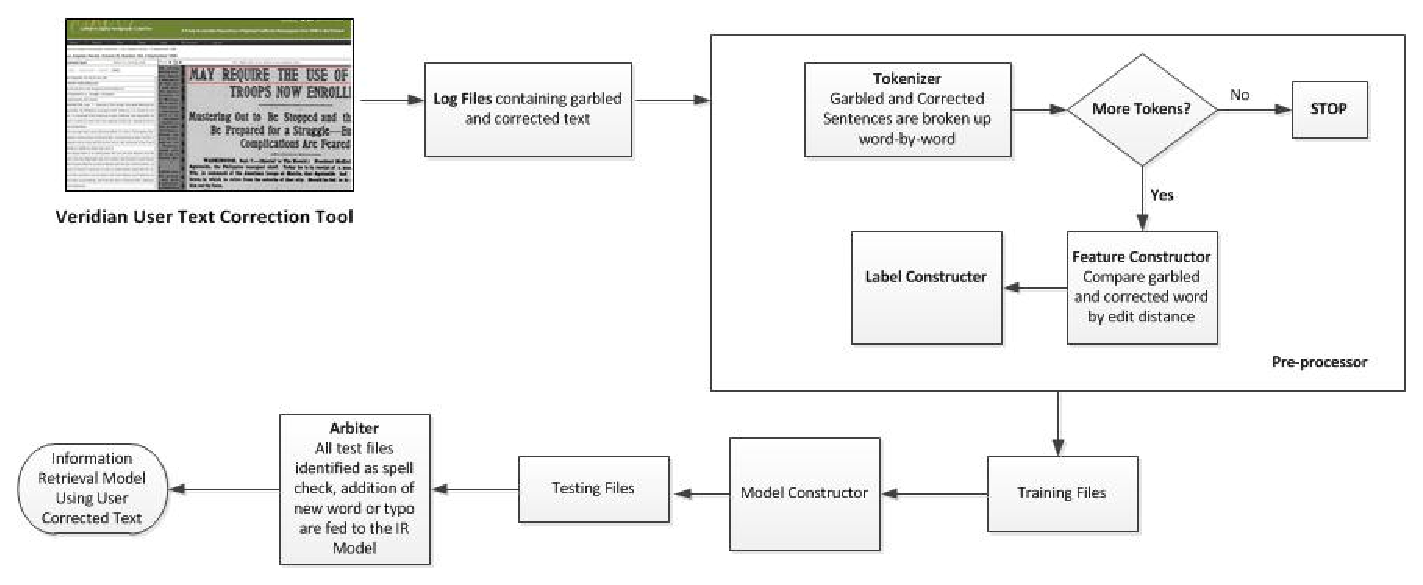
\epsfig{file=archOCR.eps, height= 3 in,width= 7 in}
\caption{The Architecture of the Proposed System}
\label{fig:arch}
\end{figure*}

\noindent \textbf{Organization}: Section~\ref{arch} describes the architecture of the proposed system; Section~\ref{sec:evaluation} presents empirical and scalability results on real-world data collected at CDNC; Section~\ref{ir} presents information retrieval techniques; Section~\ref{sec:related} discusses related work. Finally, Section~\ref{sec:conc} concludes the paper.

\section{Architecture of the Proposed System}
\label{arch}
The \textbf{C}lassification of \textbf{C}rowdsourced \textbf{T}ext \textbf{C}orrection (CCTC) system has the following components:

\begin{enumerate}

\item The \textbf{Veridian User Text Correction}\footnote{http://veridiansoftware.com/crowdsourcing/} tool which takes as input a scanned page of the newspaper and enables users to correct OCR errors as they come across them.
Figure~\ref{fig:T1}a shows an example of a scanned page from ``The Amador Ledger" published on January 26, 1900. The article to be corrected by a user is highlighted. The raw OCR text from the article and the tool used by patrons to correct text is shown in figure ~\ref{fig:T2}b.


\item \textbf{Log Files: }All corrections performed by the annotators are recorded in log files. To date approximately 1,705,149 lines have been edited by 848 annotators which resulted in 235 log files. A sample of 191 files has been used for this work. Each log file is generated at the issue-level and contains XML data about the pages in the issue. Table~\ref{table:logfile} describes the structure of the log file. The following information is provided about the corrections made by the patrons:
%\begin{enumerate}
(a) \textit{Page Id: } The id of the page in which editing was done.
(b) \textit{Block Id: } The id of the paragraph containing the line corrected by the user.
(c) \textit{Line Id: }The id of the line edited by the user.
(d) \textit{Old Text Value} is the garbled text generated by the OCR device and replaced by the user.
(e) \textit{New Text Value} is the corrected text with which the old text was replaced.
%\end{enumerate}

\begin{table}[h]
\begin{center}
\begin{tabular}{l}
\textless TextCorrectedLine lineID="P2\_TL00800"\textgreater \\
\textless OldTextValue\textgreater \textbf{Spll, Stales}\textless /OldTextValue\textgreater \\
\textless NewTextValue\textgreater \textbf{Union Stables}\textless /NewTextValue\textgreater \\
\textless /TextCorrectedLine\textgreater \\
\textless TextCorrectedLine lineID="P2\_TL00801"\textgreater \\
\textless OldTextValue\textgreater \textbf{**?�** Under Webb Hall *}\\
\textless/OldTextValue\textgreater \\
\textless NewTextValue\textgreater \textbf{Under Webb Hall} \textless/NewTextValue\textgreater \\
\textless /TextCorrectedLine\textgreater \\
\end{tabular}
\end{center}
\caption{A segment of the log file}
\label{table:logfile}
\end{table}

%\begin{figure*}[ht]
%\centering
%%\mbox{
%\subfigure[Scanned newspaper highlighting an article to be corrected by a user.]
%{
%%%\includegraphics[width=0.6\columnwidth]{odds_20070813_160000rb_M.pdf}
%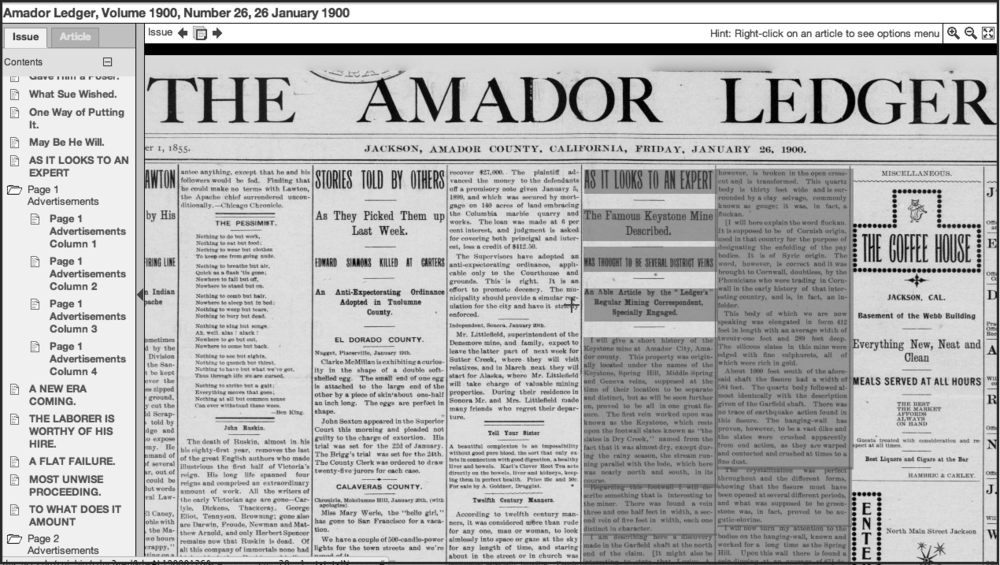
\includegraphics[width=0.48\textwidth, height=0.2\textheight]{./image/greyscale.jpg}
%\label{fig:T1}
%}
%\subfigure[The tool used by patrons to annotate articles.]
%{
%%%\includegraphics[width=0.8\columnwidth]{20070813-C1-7d-roc.pdf}
%\includegraphics[width=0.48\textwidth,height=0.2\textheight]{./image/correction.jpg}
%\label{fig:T2}
%}
%\caption{The Amador Ledger, Jan. 26, 1900.}
%\label{News_01}
%\centering
%\end{figure*}

\begin{figure*}
\centering
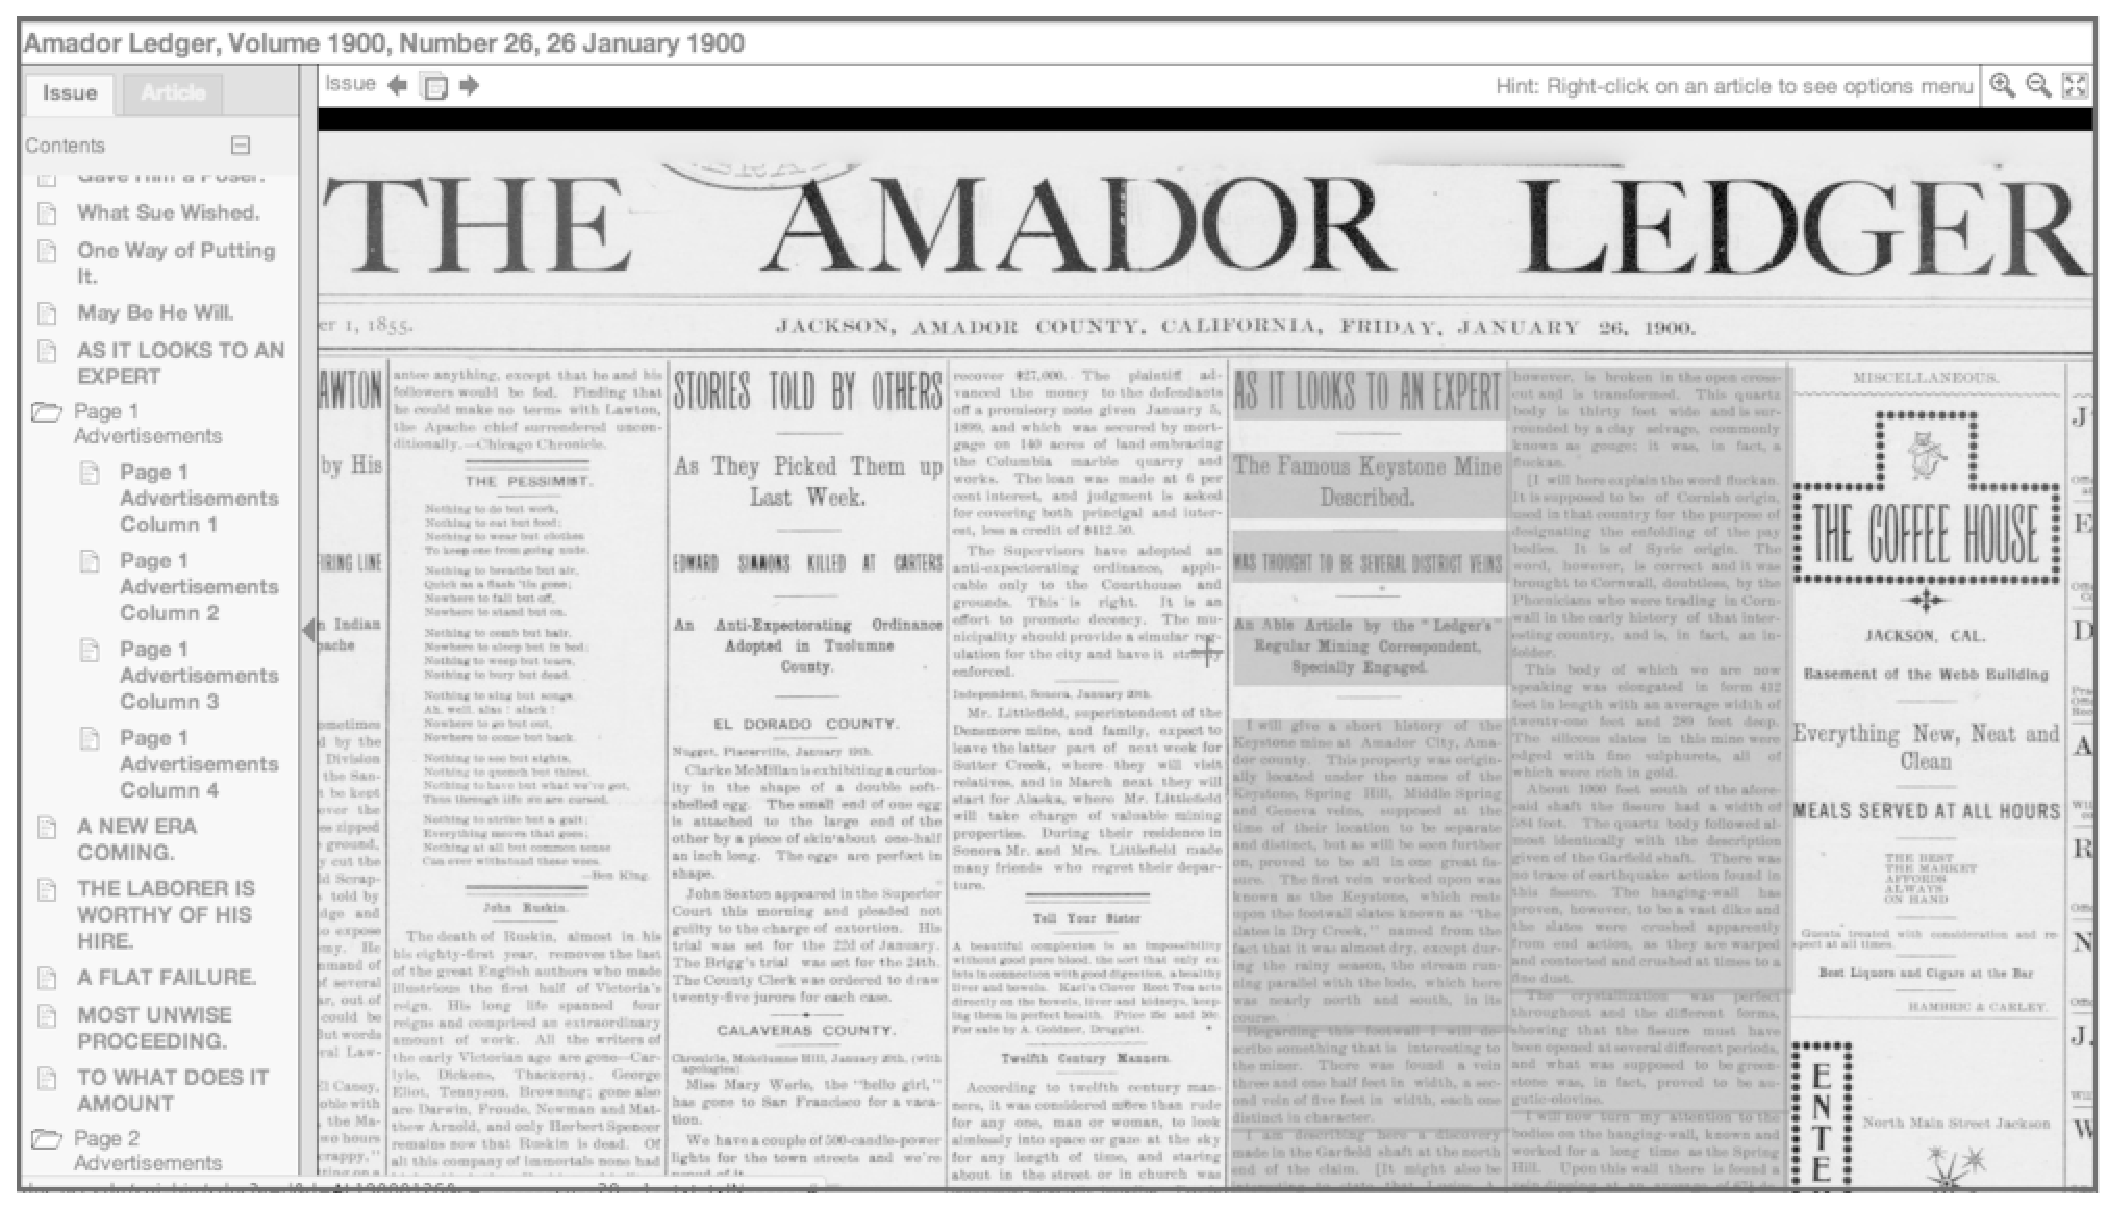
\epsfig{file=greyscale.eps, height= 1.7 in,width= 3 in}
\label{fig:T1}
\epsfig{file=correction.eps, height= 1.7 in,width= 3 in}
\label{fig:T2}
\caption{The Amador Ledger, Jan. 26, 1900}
\end{figure*}





\item \textbf{Preprocessor: } The preprocessor has three main components:
\begin{itemize}
\item \textbf{Tokenizer: } The old text and the corresponding new text from the log file is tokenized by white-spaces. There are 44,022 tokens of which 21,108 are corrected by the annotators.

\item \textbf{Feature Constructor }\\
Two different kinds of features are generated from the raw text - (1) word level and (2) character level features. Word level features are carefully crafted by hand and form the baseline for the classification task described in item~\ref{itm:mod} of Section~\ref{arch}. Character level features are automatically generated from the text corrections using machine learning algorithms. We believe these character level features will help us understand the process of automation and classification of user corrections.\\
\textbf{Word-level feature construction:}\\
Features are crafted by computing the Levenshtein edit distance between the old word and its correction. The Levenshtein edit distance \cite{Wagner_74} is defined as the minimum number of single edit operations (insertions, deletions and substitutions) required to convert one string into another. Six binary features are generated as follows: 
(a) \textbf{Difference Length Zero} : $1$, if both the old word and new word have same length and $0$ otherwise. 
%For example, the feature is 1 for the tokens ``Spll," and ``Union" as  both the tokens have same number of characters.
(b) \textbf{Difference Length Above One} : $1$, if the length of new word exceeds the length of old word and $0$ otherwise.
(c) \textbf{Edit Distance One}:  $1$, if single edit operation is required to convert old word to new word and $0$ otherwise. For example, the feature is 1 for tokens ``Under" and ``under" or ``the" and ``them".
(d) \textbf{Edit Distance Above One}: $1$, if more than one edit operation is required to convert old word to new word and $0$ otherwise. For ``Spll," and ``Union", value is 1 as more than one edit operation is required to convert from old to new token.
%(d) \textbf{Edit Distance Below Three}: 1, if less than three edit operations are required to convert old word to new word and $0$ otherwise. 
%For ``Stales" and ``Stables", value is 1 as less than three edit operations are required to convert from old to new token. 
(e) \textbf{Edit Distance is 1 and Case Change}: 1, if the two words have edit distance is exactly 1 and the first character of one string change from upper case to lower case or vice versa. For example, for ``Stales" and ``Stables", the value is 0 as there is no case change.
(f) \textbf{Punctuation Difference}: 1, if both the old text and new text differ in any of the following punctuation marks (!"\#\$\%\&'*+,-./:;\textless=\textgreater?@[$\backslash$]\^\_`\{\textbar\}\textasciitilde).

\textbf{Character-level feature construction:}\\
The tokenization process of the text in the log files was done at the character level. If the text was deleted by the user as a part of correction process then the character ``$\sim$" represented the new character denoting that the user performed the task of deletion, for example, t $\rightarrow$ $\sim$ means that the user deleted character ``t" from the old token. Whereas if the user added a new text  then the character ``+" represented that the user added text that was initially missing in the OCR data, for example + $\rightarrow$ o means that the user added character ``o" as a part of correction process. \\
The character-level dataset consists of $58,963$ instances of which we encountered that $55,612$ had same character-level corrections indicating that the OCR makes the same type of mistakes repeatedly. The maximum number of redundant corrections noted were deletion of punctuations and special characters. There were $4344$ deletions of comma, $2831$ deletions of $\ddot{A}$. Amongst character to character corrections, $635$ cases of o$\rightarrow$e, $470$ cases of b$\rightarrow$h, 299 cases of u$\rightarrow$n contributed maximum to the redundancy. The graph in figure~\ref{fig:fig3},~\ref{fig:fig4},~\ref{fig:fig5},~\ref{fig:fig6},~\ref{fig:fig7}  (See Appendix) shows that the histograms of the different character level corrections.
The x-axis in the graph denotes the examples of character-level corrections whereas the y-axis denotes the number of corrections made on the examples in the entire corpus. The performance of the proposed character level feature dataset was compared against the baseline method of manually crafted word level dataset.\\
Apriori algorithm \cite{Agrawal1994} implementation of WEKA 3.7.10 was used to mine character-level rules. Mining association rules is to discover all the strong rules in the database using different measures of interestingness. To select interesting rules from the total set of possible rules, we use some user controlled measures like minimum support ($minsup$) and minimum confidence ($minconf$). They are formally defined as follows. \\
Support(X$\rightarrow$Y) = P(X $\cup$ Y)\\
represents the percentage of instances from the database that contains both X and Y.\\
Confidence(X$\rightarrow$Y) = P(Y|X)\\ 
represents the probability that the instance containing X also contains Y.
In our case, the value of $minconf$ and the the lower bound $minsup$ was set to $0.0001$, and the upper bound of $minsup$ was set to $1$. The upper bound of $minsup$ was iteratively decreased by a factor of $delta$ until either the lower bound of $minsup$ was reached or the required number of rules were generated.\\
The number of features and instances are $6631$ and $3351$ respectively in the character-level data set.\\
\textbf{Example rules mined from the character level data}

\begin{itemize}
\item old=b ==> new=h
\item old=J  ==> new=j
\item old=K ==> new=R
 \item old=0 ==> new=6
\item old=G ==> new=6
\end{itemize}

The above examples show that the old character is corrected to a new character by the patrons. As can be seen, the transformations done by the OCR device were very close to the original word, for example, character `h' can be easily misinterpreted as character `b'.


%\begin{figure*}[t]
%\centering
%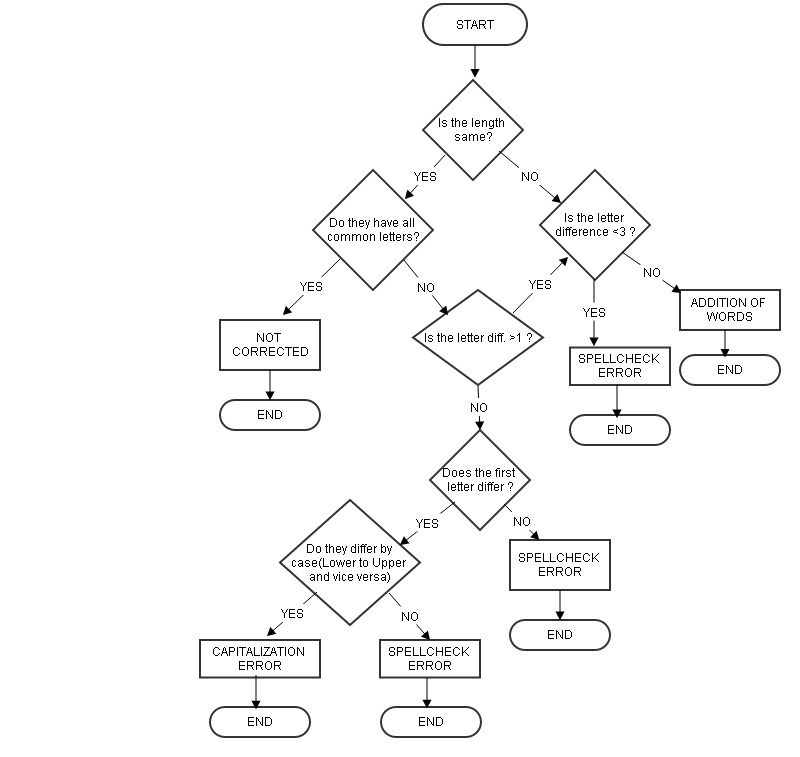
\includegraphics[width=0.9\textwidth]{./image/flowchartnew.jpg}
%%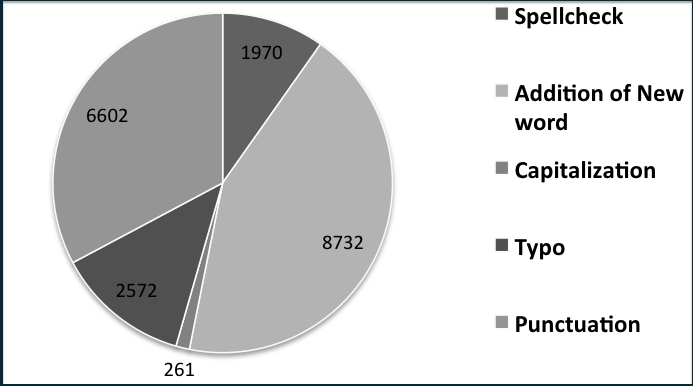
\includegraphics[width=6cm,height=4cm]{./image/error.jpg}
%\caption{Flowchart demonstrating how the labels are generated.}
%\label{fig:flowchart}
%\end{figure*}

%\begin{figure*}[ht]
%\centering
%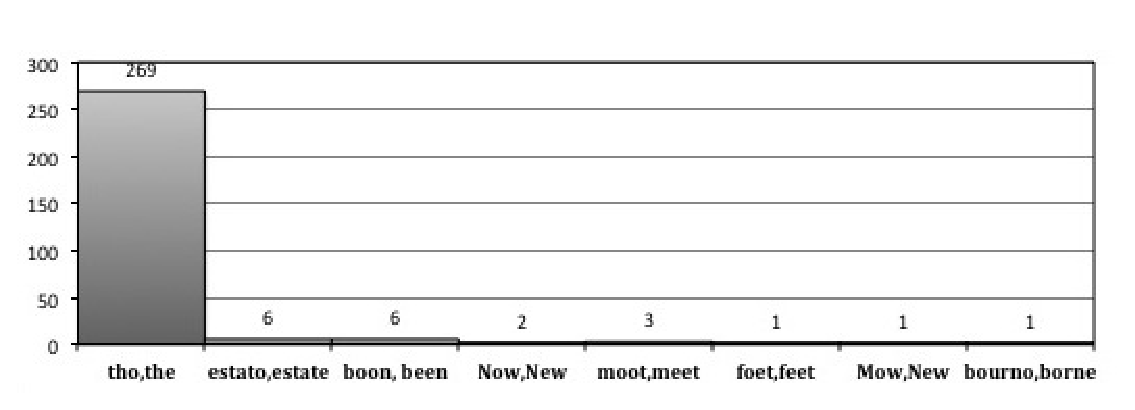
\epsfig{file=stat1edit.eps, height= 1.8 in,width= 3.4 in}
%\label{fig:stat1}
%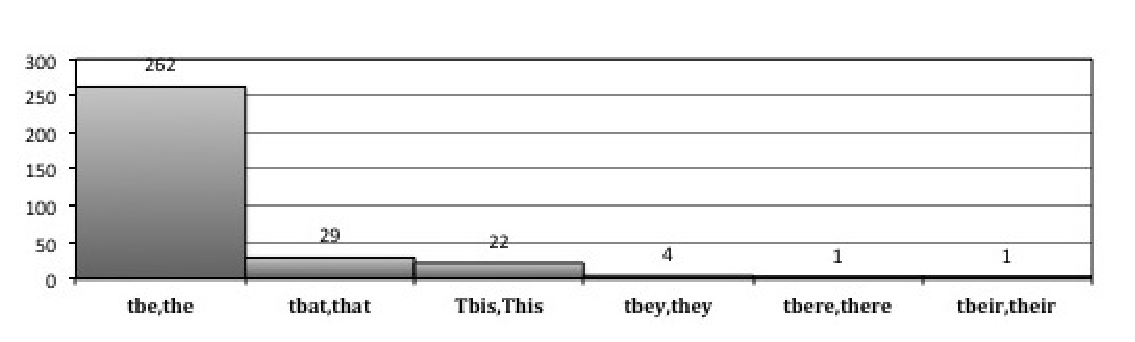
\epsfig{file=stat2copy.eps, height= 1.7 in,width= 3.3 in}
%\label{fig:stat2}
%%\epsfig{file=stat3copy.eps, height= 1.7 in,width= 3 in}
%%\label{fig:stat3}
%\caption{Examples of character level corrections}
%\end{figure*}

\item \textbf{Label Constructor: }The errors rectified by the users are categorized as addition, deletion, punctuation error, capitalization error, and spellcheck error. 
%The logic used in generation of the features can be summarized by the flowchart depicted in Figure~\ref{fig:flowchart}.
Specifically,
%\begin{enumerate}
(a) \textbf{Addition: } When the length of new string exceeds the length of old given the difference is made by alphanumeric characters and the edit distance is above one. For example, ``6RAVR" and ``GRAVEL".
(b) \textbf{Deletion: }When the length of old string exceeds the length of new given the difference is made by alphanumeric characters and the edit distance is above one. For example, ``VVe" and ``We".
(c) \textbf{Punctuation: }When the difference in the length of strings is non-zero and they differ by special characters contained in the set (!"\#\$\%\&'()*+,-./:;\textless=\textgreater?@[$\backslash$]\^\_`\{\textbar\}\textasciitilde). For example, ``Ladies!" and ``Ladies".
(d) \textbf{Capitalization: }When both the strings have equal length, edit distance is exactly 1 and first letter of both the strings change from upper to lower case or vice versa. For example, ``largest" and ``Largest".
(e) \textbf{Spellcheck: }When the difference between string is above zero and the edit distance contributed by alphanumeric character is exactly one or when the strings have same length and the edit distance is one or above one irrespective of the involvement of special characters. For example, ``the" and ``them" or ``hanger" and ``banger".

%(a)\textbf{Spellcheck Error: }When the edit distance is between 1 and 3. For example, ``mounten" and ``mountain".
%(b)\textbf{Addition of a new word: }When the edit distance is more than 3. For example, ``at" and ``attend".
%(c)\textbf{Capitalization error: } When the edit distance of two strings is exactly 1 and first letter of both the strings changes from upper to lower case or vice versa. For example, ``largest" and ``Largest".
%(d)\textbf{Typographical Error: } When the edit distance is exactly one and case change is 0. For example, ``teh" and ``the"
%(e)\textbf{Punctuation Error: }When the two strings differ by special characters contained in the set (!"\#\$\%\&'()*+,-./:;\textless=\textgreater?@[$\backslash$]\^\_`\{\textbar\}\textasciitilde). 
%%For example, ``residents" and residents
%(f)\textbf{No Correction: }When the old and new text are same. %For example, plant and plant
%%\end{enumerate}

The distribution of the these classes in the dataset is shown in Table~\ref{table: classes}. It must be noted that by design tokens are always assigned to one class, although in principle it may be possible to assign them to multiple classes\footnote{For e.g. a correction of ``t$\$$e" to ``the" could be either a Spellcheck or a Punctuation Error correction but we assign it to Spellcheck }.

\begin{table}[htdp]
\centering
\begin{tabular}{| l | l |}
\hline
 Class  & No. of Instances \\
\hline
 Addition & 4575 \\
%\hline 
Deletion & 5024 \\
%\hline
Punctuation & 6401 \\
%\hline
Capitalization & 299 \\
%\hline
Spellcheck & 4809 \\
%\aline 
\hline
Total & 21108 \\
\hline
\end{tabular}
\caption{Class Distribution}
\label{table: classes}
\end{table}
\end{itemize}

%\begin{figure}[h]
%\centering
%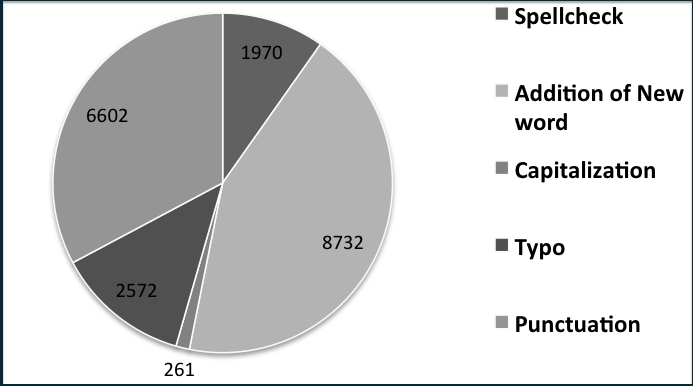
\includegraphics[width=0.48\textwidth]{./image/error.jpg}
%%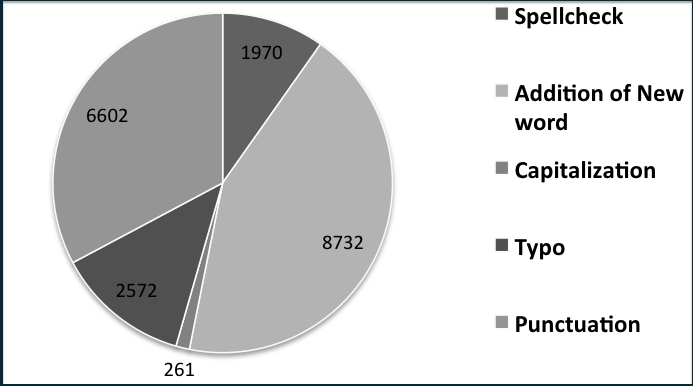
\includegraphics[width=6cm,height=4cm]{./image/error.jpg}
%\caption{Error Classification}
%\label{fig:stats}
%\end{figure}

%The dataset was parsed to a format used by the Joachim's multi class SVM algorithm which is represented as\\
%\textless target\textgreater\space\textless feature\textgreater:\textless value\textgreater ......\textless feature\textgreater:\textless value\textgreater\\
%The number of instances in the dataset is 44,022. 
%The class distribution in the dataset is shown in table ~\ref{table: classes}

%\item \textbf{Baseline Character-Level Feature Construction: }
%The tokenization process of the text in the log files was modified to enable the addition and deletion classification of text using a character. If the text was deleted by the user as a part of correction process then the character ``$\sim$" was assigned to the new token denoting that the user performed the task of deleting the OCR garbled text whereas if the user added a new text  then the character ``+" was assigned to the old token denoting that user added text that was initially missing in the OCR data. All the corrected tokens were further split into character level data with the tuple \textless old char, new char\textgreater  replacing the previous token level notion of \textless old token,new token\textgreater giving us $58,963$ instances of data. Of $58,963$ instances, we encountered that $55,612$ instances were redundant which signifies that the OCR device makes the same type of mistakes repeatedly. The maximum number of redundant corrections noted were deletion of punctuations and special characters. There were $4344$ deletions of comma, $2831$ deletions of $\ddot{A}$. Amongst character to character corrections, $635$ cases of o$\rightarrow$e, $470$ cases of b$\rightarrow$h, 299 cases of u$\rightarrow$n contributed maximum to the redundancy. Hence, the number of unique instances was found to be $3351$. Figure ~\ref{fig:stat1}a and ~\ref{fig:stat2}b shows histograms of few o$\rightarrow$e and b$\rightarrow$h corrections made by users. In order to test the performance of the manually crafted features of the dataset, we automatically generated rules using apriori algorithm to mine association rules. Mining association rules means to find all association rules that have support and confidence greater than or equal to user specified minimum support ($minsup$) and minimum confidence ($minconf$) respectively. In our case, the value of $minconf$ and the the lower bound $minsup$ was set to $0.0001$, and the upper bound of $minsup$ was set to $1$. The upper bound of $minsup$ was iteratively decreased by a factor of $delta$ until either the lower bound of $minsup$ was reached or the required number of rules were generated. The number of rules generated by the algorithm were $6631$.

%%Some of the user defined parameters used in the algorithm are support and confidence. Support, sup(o$\rightarrow$e) is defined as the probability that letter `o' gets replaced to letter `e'. And confidence, conf(o$\rightarrow$e) is defined as the probability that the new character is `e' given the old character is `o'.
%%minimum confidence, was set to 1.0E-4, delta:  1.0E-4, upper bound minimum support: 1.0, lower bound minimum support: 1.0E-4.



%The error labels are the same as that for token level data.
%(a) \textbf{Addition: } When a user inserts a new token `T' in place of void, the old character is assigned a symbol `+'. For example, + $\rightarrow$ T.
%(b) \textbf{Deletion: } When a user removes an existing token `A' from the old text, the new character is assigned a symbol `$\sim$'. For example, A $\rightarrow$ $\sim$.
%(c) \textbf{Capitalization error: } When an old character is capitalized or decapitalized to form a new character. For example, l $\rightarrow$ L.
%(d) \textbf{Punctuation error: } When a substitution of an old to new character involves a punctuation. For example, ! $\rightarrow$ t.
%(e) \textbf{Spellcheck error: } When an old alphanumeric character is replaced by a new alphanumeric character. For example, o $\rightarrow$ e.

%\begin{figure*}[ht]
%\centering
%\subfigure[o changed to e]
%{
%%%\includegraphics[width=0.8\columnwidth]{20070813-C1-7d-roc.pdf}
%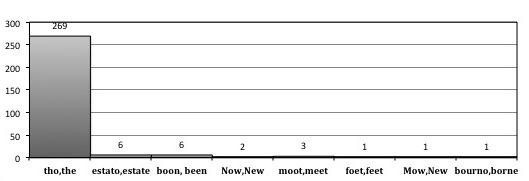
\includegraphics[width=0.45\textwidth, height=0.13\textheight]{./image/stat1edit.jpg}
%\label{fig:stat1}
%}
%\subfigure[b changed to h]
%{
%%%\includegraphics[width=0.8\columnwidth]{20070813-C1-7d-roc.pdf}
%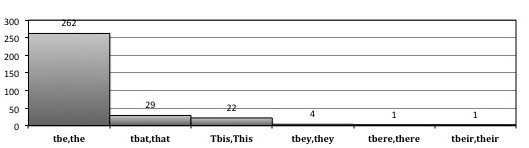
\includegraphics[width=0.45\textwidth,height=0.13\textheight]{./image/stat2copy.jpg}
%\label{fig:stat2}
%}
%\subfigure[u changed to n]
%{
%%%\includegraphics[width=0.6\columnwidth]{odds_20070813_160000rb_M.pdf}
%\includegraphics[width=0.33\textwidth,height=0.13\textheight]{./image/stat3copy.jpg}
%\label{fig:stat3}
%}
%\caption{Example of character level corrections}
%\label{News_01}
%\end{figure*}




\item \label{itm:mod} \textbf{Model Construction: } The model for classifying crowdsourced text correction is built using a Multiclass Support Vector Machine algorithm \cite{Tsochantaridis_2004}. Each training point belongs to one of $k$ different classes. The goal is to construct a function, which given a new data point, will correctly predict the class to which it belongs.
Different methods have been proposed in literature for solving the SVM multi-class classification problem. Some popular techniques include: a) \textit{One-Versus-All (OVA) classification} Build $k$ different binary classifiers; for the $i^{th}$ classifier, let the positive examples be all points in class $i$ and negative examples not in class $i$. Let $f(x) = \text{arg } max_i f_i(x) $.  b) \textit{one-versus-one} uses the majority voting strategy where each classifier assigns the new instance one of two classes. The class with the majority votes is assigned to the instance.
%%It generates k(k-2)/2 models for a k class problem. This approach is not practical for large-scale classification because of the memory required for storing k(k-1)/2 models.
%c) \textit{Directed Acyclic Graph SVM} in its training phase, it is the same as the one-vs-one method. However, in the testing phase, it uses a rooted binary directed acyclic graph which has k(k-1)/2 internal nodes and k leaves. 
%d) \textit{Error Correcting Output Codes} \cite{multiclassSVM_ecoc} This technique tries to combine binary classifiers by using decorrelations and correct errors.
Crammer and Singer \cite{crammer} pose the multi-class classification problem as a single optimization problem, rather than decomposing it into multiple binary classification problems. A comparison of the above approaches can be found here \cite{comparison}.

For a training set $(x_1,y_1) ... (x_n,y_n)$ with labels $y_i \in \{1, \cdots, k\}$, the multi class problem can be posed as a constrained optimization problem with a quadratic objective function:
$\text{min } \frac{1}{2} \sum_{i = 1}^{k} \parallel w_{i}\parallel^2 + \frac{C}{n} \sum_{i = 1}^{n}\xi_{i} $

s.t. $\forall y \leq k : [x_{1} \cdot w_{yi}] \geq [x_{1} \cdot w_{y}] + 100*\Delta(y_{1},y)-\xi_{1}$
$\cdots$
s.t. $\forall y \leq k : [x_{n} \cdot w_{yn}] \geq [x_{n} \cdot w_{y}] + 100*\Delta(y_{n},y)-\xi_{n}$

Here $C$ is the regularization parameter, $\Delta(y_{j},y), 1 \le j \le n$ is the loss function that returns 0 if $y_{j}$ equals y, and 1 otherwise and $\xi_{i}, 1 \le i \le n$ are the non negative slack variables which measure the degree of misclassification of the instance $x_{i}$. 
%\cite{algo} has to two modules, \textit{svm\_multiclass\_learn} and \textit{svm\_multiclass\_classify}. The learning module learns the model given the parameters and the training data whereas the classification module applies the learned model to the test data to find the error. 
It must be noted that when the data is not linearly separable, the following kernel functions are used for classification:
%the original finite dimensional space is mapped to a much higher dimensional space in order to make the separation easier in that space. The mappings used by SVM schemes are designed to ensure that the dot products may be computed easily in terms of the variables in the original space, by defining them in terms of a Kernel function selected to suit the problem. The types of kernel function used can be described as follows:\\
a) Linear Kernel: $K(x,y) = x^{T}y + c $
b) Polynomial Kernel : $K(x,y) = (\alpha x^{T}y + c)^{d}$
c) Radial Basis Kernel : $K(x,y) = exp(-\lvert \lvert x-y\rvert\rvert^{2}/2\sigma^{2}$)


\begin{table*}
\parbox{.51\linewidth}{
\centering
\begin{tabular}{|lllll|}
\hline
C &$AE_{p}$&$AE_{b}$&$AT_{p}$&$AT_{b}$\\
\hline
.0001&99.43$\pm .09$&49.47$\pm0.25$&1.268$\pm.06$&0.11$\pm.01$\\
.1&99.43$\pm .09$&49.464$\pm .47$&2.512$\pm0.01$&0.061$\pm0.01$\\
10&99.43$\pm .09$&4.974$\pm .5$&2.512$\pm0.01$&0.17\\
1000&99.43$\pm .09$&1.743$\pm .14$&3.635$\pm0.08$&0.382$\pm0.04$\\
10000&99.43$\pm .09$&0&6.126$\pm0.02$&0.303$\pm0.02$\\
\hline
\end{tabular}
\caption{Results using linear kernel}
\label{table: error}
}
\hfill
\parbox{.51\linewidth}{
\centering
\begin{tabular}{|l|ll|ll|}
\hline
&Polynomial&&RBF&\\
\cline{2-5}
C&$AE_{p}$ & $AE_{b}$&$AE_{p}$&$AE_{b}$\\
\hline
.0001&42$\pm.13$&50$\pm.47$&63$\pm.15$&27$\pm.5$\\
100&42$\pm.13$&.33$\pm.2$&63$\pm.16$&3$\pm.4$\\
1000&42$\pm.13$&0$\pm0$&63$\pm.16$&1.7$\pm.2$\\
\hline
C&$AT_{p}$ & $AT_{b}$ &$AT_{p}$ & $AT_{b}$ \\
 \hline
.0001&37$\pm1.4$&10$\pm0.2$&25$\pm0.7$&6$\pm0.2$\\
100&326$\pm11.8$&1239$\pm118$&$540\pm110$&404$\pm34$\\
1000&942$\pm17.4$&764$\pm93$&537$\pm111.72$&957$\pm184$\\
\hline
\end{tabular}
\caption{Results using polynomial and rbf kernels}
\label{table: kernels}
}
\end{table*}



\item \textbf{Information Retrieval Techniques: } The tokens identified by the model as ``spell check",``addition", ``capitalization", and ``punctuation" play an important role in trying to enhance search and retrieval on the archive. This is presented here for the completeness of the architecture, but described in detail in Section~\ref{ir}.

\end{enumerate}

\section{Empirical Evaluation}
\label{sec:evaluation}
The goal of our experiments is to understand whether character level features or word level features are better predictors of the class of text correction.
The experiments are performed on a linux HPC cluster with 20 CPU(s) and 10 cores per socket, 99GB RAM and 2.50GHz of processor speed. In these experiments, the regularization parameter $C$ is varied from $0.0001$ to $10000$ for the linear kernel. The performance of the algorithm is evaluated using 10-fold cross validation technique. The \textbf{A}verage (loss) \textbf{E}rror (AE) and  \textbf{A}verage (running) \textbf{T}ime (AT) from cross validation for baseline (word-level) and proposed (character-level) dataset respectively are represented as $AE_{b}$, $AE_{p}$. Table ~\ref{table: error} shows the result of the experiment, error and running time (cpu seconds) using linear kernel for different values of $C$. Table~\ref{table: kernels} shows the result of the experiment, error and running time (cpu minutes) using polynomial and radial basis kernel. As it can be seen from the results, the word level features perform better than the character level.\\
The multi-class SVM algorithm using polynomial kernel gives the best results in both the datasets, word-level and character-level. In case of automatically generated character-level dataset, the performance of the algorithm does not improve by varying the regularization constant in contrast to the performance of the manually crafted word-level dataset. In case of word-level dataset, as the value of regularization constant increases, the average loss of the learning model decreases. However, the time taken to train the model is considerably high. It must also be noted that one can learn less accurate but faster models with linear or RBF kernels. Thus, it may be useful to consider a trade-off between accuracy of learnt models versus time taken for classification in large scale deployments.
 
The code used to build the prototype system along with data generated are available at the github account\footnote{https://github.com/megha89/}. It must be noted that the $SVM^{multiclass}$V2.2 package \cite{algo} was used for the implementation of Multi-class SVMs. 
For linear kernels, $SVM^{multiclass}$V2.20 is very fast and runtime scales linearly with the number of training examples. Training of non-linear kernels is very slow using the algorithm described in Section~\ref{arch}.

%\subsection{Results}
%\begin{table}
%\begin{center}
%\begin{tabular}{|lllll|}
%\hline
%C &$AE_{b}$&$AE_{p}$&$AT_{b}$&$AT_{p}$\\
%\hline
%.0001&99.43$\pm .09$&49.47$\pm0.25$&1.268$\pm.06$&0.11$\pm.01$\\
%.1&99.43$\pm .09$&49.464$\pm .47$&2.512$\pm0.01$&0.061$\pm0.01$\\
%10&99.43$\pm .09$&4.974$\pm .5$&2.512$\pm0.01$&0.17\\
%1000&99.43$\pm .09$&1.743$\pm .14$&3.635$\pm0.08$&0.382$\pm0.04$\\
%10000&99.43$\pm .09$&0&6.126$\pm0.02$&0.303$\pm0.02$\\
%\hline
%\end{tabular}
%\caption{Experiment results using linear kernel}
%\label{table: error}
%\end{center}
%\end{table}
%
%\begin{table}[htdp]
%\begin{tabular}{|l|ll|ll|}
%\hline
%&Poly&&RBF&\\
%\cline{2-5}
%C&$AE_{b}$ & $AE_{p}$&$AE_{b}$&$AE_{p}$\\
%\hline
%.0001&42$\pm.13$&50$\pm.47$&63$\pm.15$&27$\pm.5$\\
%100&42$\pm.13$&.33$\pm.2$&63$\pm.16$&3$\pm.4$\\
%1000&42$\pm.13$&0$\pm0$&63$\pm.16$&1.7$\pm.2$\\
%\hline
%C&$AT_{b}$ & $AT_{p}$ &$AT_{b}$ & $AT_{p}$ \\
% \hline
%.0001&37$\pm1.4$&10$\pm0.2$&25$\pm0.7$&6$\pm0.2$\\
%100&326$\pm11.8$&1239$\pm118$&$540\pm110$&404$\pm34$\\
%1000&942$\pm17.4$&764$\pm93$&537$\pm111.72$&957$\pm184$\\
%\hline
%\end{tabular}
%\caption{Experiment Results using polynomial and rbf kernels}
%\label{table: kernels}
%\end{table}


%\subsection{Discussion}
%\subsection{Known Defects}
%The \cite{algo} algorithm converges quickly for linear type kernel but the its performance on test set is poor. For non linear kernels, this algorithm does not scale well for large scale datasets but gives better performance than linear kernels.
\section{Information Retrieval \\Techniques}
\label{ir}
The following details are relevant: 

\noindent \textbf{Query Set:} To measure the retrieval effectiveness of the corrected text versus the garbled OCR, a list of 20 keywords for search was prepared by randomly sampling from the corrected words. The table~\ref{table:keywords} (See Appendix) presents the list of 20 keywords that were used to analyse the retrieval effectiveness of raw OCR versus corrected OCR text.

\noindent \textbf{Software:} PyLucene 3.6.2, a Python extension for accessing Java Apache Lucene was used as an IR software library for enabling full text indexing and search capabilites. Inverted indices are built for both the original and corrected corpus. Keywords from the query set are tested on both corpora and documents containing words in the query set are retrieved. The documents are ranked according to the frequency of the keyword present -- higher the frequency, higher the rank.

\noindent \textbf{Evaluation:} The main aim of this system is to improve the quality of text for use with an IR system. The metric used for evaluation here is mean reciprocal rank (MRR) \cite{manning2008introduction} which produces a list of possible ranked responses to a sample of queries, Q. The reciprocal rank is the multiplicative inverse of the rank of the first correct answer. The first correct answer is decided by the users. The average of the reciprocal ranks over a sample of queries is the mean reciprocal rank.
MRR = $\frac{1}{|Q|} \sum_{i = 1}^{|Q|} \frac{1}{rank_{i}}$

The same set of queries were applied on both the datasets, that is raw OCR and corrected OCR individually. For each of the of $20$ queries, we chose the most relevant document from the retrieved results and observed the rank of the most relevant document in both the set of results. The MRR for the raw OCR data was noted to be $0.355$ whereas for corrected data it was $0.65415$. The higher value of MRR denotes that relevant results get higher priority in corrected corpus. The metric MRR was chosen because it did not require relevance feedback from the users as in precision/recall \cite{manning2008introduction}.

 
%\noindent \textbf{Evaluation:} The main aim of this system is to improve the quality of text for use with an IR system. The metric used for our evaluation include the standard IR techniques of recall and precision. Recall is defined as the ratio of number of relevant documents returned to the total number of relevant documents for a query, in the collection. Precision is defined as the ratio of number of relevant documents returned to the total number of documents returned for a given query. The document to query relevance is manually determined by other computer science students. The table shows the precision at ten standard recall points for corrected OCR text over the raw OCR text.  

%The metric used to compare the retrieved documents is Spearman's rank correlation coefficient($\rho$). Let $y_{i}$ be the rank ordering of the documents retrieved from the corrected corpus and $x_{i}$ the rank ordering for the garbled text. Let $d_{i}$ = $x_{i}$ - $y_{i}$. Then Spearman's rank correlation $\rho$ is given by: $\rho = 1 - \frac {6\sum d_i^2 }{n(n^2-1)}$.

%\noindent \textbf{Example: } Query word ``Jackson", the evaluation of $\rho$ is shown in Table~\ref{ex}. Here, ${\sum d_i^2}$ = 11 and $\rho$ = 0.45.
%\begin{table}[h]
%\centering
%\begin{tabular}{ l | c | c | c | r | r }
% $Y_{i}$ & $X_{i}$ & $y_{i}$ & $x_{i}$ & $d_{i}$ & $d_{i}^2$ \\
%\hline
%  12-01-1900 & 21-10-1910 & 1 & 10(4) & -3 & 9 \\
%  09-12-1910 & 09-12-1910 & 2 & 2(1) & 0 & 0 \\
%  08-06-1900 & 23-09-1910 & 3 & 7(2) & 1 & 1 \\
%  01-04-1904 & 02-12-1910 & 4 & 8(3) & 1 & 1 \\
%  25-05-1900 & 23-12-1910 & 5 & 11(5) & 0 & 0 \\
%\end{tabular}
%\label{ex}
%\end{table}

\noindent \textbf{Deployment: }The full-scale deployment of this prototype system is being considered on old historic newspaper archives at California Digital Newspaper Collection and the New York Public Library among others, where  user text corrections are used extensively for cleaning garbled OCR. 

\section{Related Work}
\label{sec:related}
\noindent \textbf{Optical Character Recognition (OCR)} is a commonly used method of digitizing printed texts so that it can be searched and displayed online, stored compactly and used in text mining applications. The text generated from OCR devices is often garbled due to variations in quality of the input paper, size and style of the font and column layout, its condition at the time of microfilming, choice of scanner, and the quality of the OCR software. Several techniques for post processing garbled OCR have been designed \cite{Fujisawa_08}, \cite{Esakov_94}, \cite{Lecun_90}. These include:

\noindent \textbf{Dictionary based schemes: }These algorithms use a dictionary to spellcheck misspelled OCR recognized words. They correct non-word errors - words that are recognized by the OCR device but do not correspond to any entry in the lexicon. Niwa et al. \cite{postprocessing} proposed an OCR post error correction method based on pattern learning where a list of suitable candidates is generated from the lexicon and the best candidate is selected as a correction. Yannakoudakis and Fawthrop \cite{Yannakoudakis_83} conducted a study to create a set of rules based on common misspelling pattern and used them to correct errors. Cherkassky and Vassilas \cite{Cherkassky_89} use back propagation algorithms for correction. 
%\cite{statistical} proposed using Hidden Markov Models (HMMs) to integrate syntactic information into the post-processing error correction. 
%The suggested model achieved a higher rate of error correction due to its statistical nature in selecting the most probable candidate for a particular misspelled word.

\noindent \textbf{Context based schemes: }These algorithms perform error detection and correction based on the grammatical error and semantic context. They are able to correct real-word errors -- words that are recognized by the OCR system and correspond to an entry in the lexicon. Tong and Evans \cite{Tong96astatistical} describe an automatic, context-sensitive, word-error correction system based on Statistical Language Modeling (SLM). The system exploits information from letter n-grams, character confusion probabilities and word bi-gram probabilities. Golding et al. \cite{contextbased} applies a part-of-speech (POS) tagger enhanced by word trigram model and a statistical Bayesian classifier to correct real-word errors in OCR text. Reynaert \cite{Reynaert2008a} presents a system for reducing the level of OCR-induced typographical variation in large text collections called Text-Induced Corpus Clean-up (TICCL). The system focuses on high-frequency words to be cleaned and gathers all typographical variants for any particular focus word that lie within the predefined Levenshtein distance. Bassil et al. \cite{Bassil_12a,Bassil_12b} propose a post-processing context-based error correction algorithm for detecting and correcting OCR non-word and real-word errors. The proposed algorithm is based on Google's online spelling suggestion. Abdulkader et al. \cite{lowcost}  present a method for digitizing textual data by using neural network classifiers to estimate OCR errors, clustering similar errors, designing a user interface and using active learning to tune the error estimation from user labeled data. 
Velagapudi \cite{velagapudi} uses a combination of classifiers -- kNN classifier,  multilayer perceptrons and SVM to discuss the effects of error correction on the classification accuracy of each method. 

Very little work has been done on automatic \emph{classification} of OCR error corrections\footnote{Most prior work has dealt with evaluation of candidate corrections for OCR errors.} to get a clear understanding of the \emph{nature} of errors encountered -- Esakov et al. \cite{Esakov_94a} suggest classification of output from the OCR engine as simple substitutions ($e \rightarrow c$), improper segmentation or multiple substitutions $(T \rightarrow 'l, m \rightarrow rn, he \rightarrow b)$, deletions and insertions (involving space) and unrecognized characters $(u \rightarrow \sim)$. They use a new variant of the dynamic programming algorithm for classification. In \cite{hybred}, OCR documents are classified into fixed number of categories based on their content. The accuracy of their approach was best when evaluated using SVM among other algorithms. Daoason \cite{Jon_12} posits that OCR errors are not random -- for example, it is extremely unlikely that the letter $o$ will be misrecognized as $x$ since they are very dissimilar. He classifies OCR errors as character errors (characters in the input document that are replaced with other characters), word errors (word in the input document is not correct or not present in the OCR generated text), or zoning errors (OCR software is unable to decipher zones correctly). Our work primarily focusses on \emph{manual} error correction classification where the task of correcting OCR errors is outsourced to a crowd of workers. 
%By engaging a large crowd of people for ideas, skills or participation the quality of work done is superior and relatively inexpensive.

%It is estimated that the total count of published books in the world is around 130 million \cite{bookscount}. Many of these books published are only available in printed format due to reasons like copyright and licensing issues. This limits the search of these articles, their availability and accessibility on the web. As of 2013, more than 30 million books have been digitised by Google Books Library Project \cite{gblp}. It uses reCAPTCHA to digitise books one word at a time by sending words that can not be read by the computer to the web in the form of CAPTCHAs for humans to decipher \cite{recaptcha}. 

%The OCR enables searching of full text data but it is not 100\% accurate. Its accuracy largely depends on paper quality of the original issue, font style, column layouts, its condition at the time of microfilming, choice of scanner \cite{issue}, and the quality of the OCR software. The OCR errors are widely classified as non-word errors and real-word errors. A non-word error takes place when the erroneous word is not a dictionary word whereas in real-word error the erroneous word is correctly spelt and therefore can be found in the dictionary but incorrectly used in context.
%The error generated by OCR can be classified in several categories. One such classification similar to ours is done by \cite{post-correction}. It gives an exhaustive error classification that helps in classifying real words , that is words that are not contained in any of the dictionary, e.g. names, out-dated or historic spelling variations. Segmentation errors, Hyphenation error, Misrecognition of characters, Punctuation errors, Case sensitivity, Changed word meaning are the classes required for better classification of OCR errors.

%The OCR errors are usually dependent on some major factors like the page quality, text layout, font styles. In \mydoubleq{Issues in automatic error correction}, the experimental analysis has shown that there is another important factor that impacts the performance of the OCR errors which is the choice of scanners used to scan the printed text. The type of scanner used not only affect the quantity of errors but quality as well. Their algorithm for classifying OCR errors is based minimising the cost of basic operations used to transform one string to another, also known as edit distance using dynamic programming approach.\\
%\mydoubleq{Unsupervised Post Correction} paper talks about the post processing of OCR text to minimise the errors. It uses a combination of Anagram Hashing techniques, bigram approach on word level to consider the context and a  similarity key technique called OCR-key.  Anagram Hashing technique uses a hashing function that assigns same number to all those words that have same characters. OCR key observes the shape of characters to know the nature of OCR system and its generated errors.
\noindent \textbf{Crowdsourced OCR correction }Recruiting users and paying them small sums of money to tag and annotate text and images in large digital archives has become common practice (e.g. Amazon's Mechanical Turk, reCAPTCHA \cite{vonAhn_08}, ESP \cite{vonAhn_04}) and Games with a Purpose \cite{Ahn_08w}. A number of recent papers have evaluated the effectiveness of using Mechanical Turk to create annotated data for text and natural language processing applications \cite{Snow_08}. In the same vein, many workshops and conferences have been organized on the theme of machine learning in human computation, crowdsourcing and collective intelligence\footnote{See http://ir.ischool.utexas.edu/crowd/}. 

Intuitively, the easiest way to correct garbled OCR text is to hire a group of people to edit it manually. Distributed Proofreaders (DP) \cite{DP} is a web-based project designed to facilitate proofreading of paper books into e-books and was meant to assist the project Gutenberg\footnote{http://www.gutenberg.org/}. Wikipedia is yet another example of a large scale crowdsourcing project. Yamangil et al. \cite{wikiedits} proposed a learning algorithm for mining wikipedia edit history using baseline Hidden Markov Model augmented with perceptron re-ranking. The model was trained on wikipedia edits and hence incorporated human corrections. 
%\subsection{Multi-class SVM}



\section{Conclusion \& Future Work}
\label{sec:conc}
The California Digital Newspaper Collection has an archive of 400,000 pages of historical California newspapers published between 1846 to 1922. This archive which has been subjected to OCR is currently stored in an online database accessible to the patrons. The OCR scanning process generates lot of garbled text which needs to be corrected to make the online newspaper repository more accessible to general public. 

In this paper, we present a system for Classification of Crowdsourced Text Correction which is capable of modelling user corrections using state-of-the-art machine learning techniques and retrieve categories which are likely to enhance search on the archive such as addition of words, elimination of typographical errors or addition of content. We also compared the two datasets, word-level and character-level by applying the machine learning algorithms on each. The manually crafted word-level dataset performed better in terms of average loss error. However, the running time of the algorithm was considerably high. Thus, there is a need to improve the algorithms in order to make them compatible with large scale datasets.\\
Information retrieval metric, mean reciprocal rank is used to quantify the effectiveness of the user text correction. The higher value of the MRR in the case of corrected corpus indicates that the relevant results are ranked higher in the retrieved set of documents. The prototype system is being considered for deployment on historic newspaper archives at the California Digital Newspaper Collection and the New York Public Library.

% use section* for acknowledgement
\section*{Acknowledgment}
This work is supported by funding from the National Endowment for Humanities, Grant No: NEH HD-51153-10. The authors would like to thank Stefan Boddie, DL Consulting, Ltd., New Zealand for sharing experiences with the Veridian software and Luis. C. Baquera, University of California, Riverside for providing data generated from the log files at CDNC.\\

%\bibliographystyle{IEEEtran}
%\bibliographystyle{abbrv}
%\bibliography{sig-alternate}
\bibliographystyle{abbrv}
\bibliography{sig-alternate}  % sigproc.bib is the name of the Bibliography in this case
%\begin{table*}
%\centering
%\caption{Some Typical Commands}
%\begin{tabular}{|c|c|l|} \hline
%Command&A Number&Comments\\ \hline
%\texttt{{\char'134}alignauthor} & 100& Author alignment\\ \hline
%\texttt{{\char'134}numberofauthors}& 200& Author enumeration\\ \hline
%\texttt{{\char'134}table}& 300 & For tables\\ \hline
%\texttt{{\char'134}table*}& 400& For wider tables\\ \hline\end{tabular}
%\end{table*}
%% end the environment with {table*}, NOTE not {table}!
%
%\subsection{Figures}
%Like tables, figures cannot be split across pages; the
%best placement for them
%is typically the top or the bottom of the page nearest
%their initial cite.  To ensure this proper ``floating'' placement
%of figures, use the environment
%\textbf{figure} to enclose the figure and its caption.
%
%This sample document contains examples of \textbf{.eps}
%and \textbf{.ps} files to be displayable with \LaTeX.  More
%details on each of these is found in the \textit{Author's Guide}.
%
%\begin{figure}
%\centering
%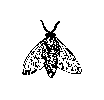
\epsfig{file=fly.eps}
%\caption{A sample black and white graphic (.eps format).}
%\end{figure}
%
%\begin{figure}
%\centering
%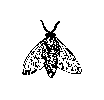
\epsfig{file=fly.eps, height=1in, width=1in}
%\caption{A sample black and white graphic (.eps format)
%that has been resized with the \texttt{epsfig} command.}
%\end{figure}
%
%
%As was the case with tables, you may want a figure
%that spans two columns.  To do this, and still to
%ensure proper ``floating'' placement of tables, use the environment
%\textbf{figure*} to enclose the figure and its caption.
%and don't forget to end the environment with
%{figure*}, not {figure}!
%
%\begin{figure*}
%\centering
%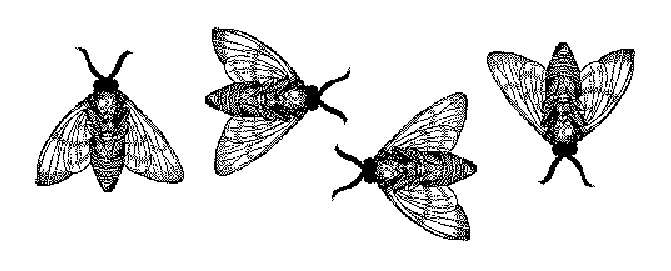
\epsfig{file=flies.eps}
%\caption{A sample black and white graphic (.eps format)
%that needs to span two columns of text.}
%\end{figure*}
%
%Note that either {\textbf{.ps}} or {\textbf{.eps}} formats are
%used; use
%the \texttt{{\char'134}epsfig} or \texttt{{\char'134}psfig}
%commands as appropriate for the different file types.
%
%%\begin{figure}
%%\centering
%%\psfig{file=rosette.ps, height=1in, width=1in,}
%%\caption{A sample black and white graphic (.ps format) that has
%%been resized with the \texttt{psfig} command.}
%%\vskip -6pt
%%\end{figure}
%%APPENDICES are optional
%\balancecolumns

\appendix
\begin{table*}[th]
\centering
\begin{tabular}{| l | l |}
\hline
 S.no  & Keywords\\
\hline
1 & prices\\
2 & trade \\
3 & character \\
4 & Development \\
5 & Aldrich \\
7 & Sutter \\
8 & south \\
9 & Sacramento \\
10 & compelled \\
11 & insertion \\
12 & estate \\
13 & Pacific \\
14 & missed \\
15 & cough \\
16 & kidneys \\
17 & CALAVERAS \\
18 & sheep \\
19 & aces \\
20 & controlled \\
\hline
\end{tabular}
\caption{List of keywords containing upper and lower case words, randomly sampled from the corrected corpus are used for testing the information retrieval techniques.}
\label{table:keywords}
\end{table*}

\begin{figure*}[ht]
\centering
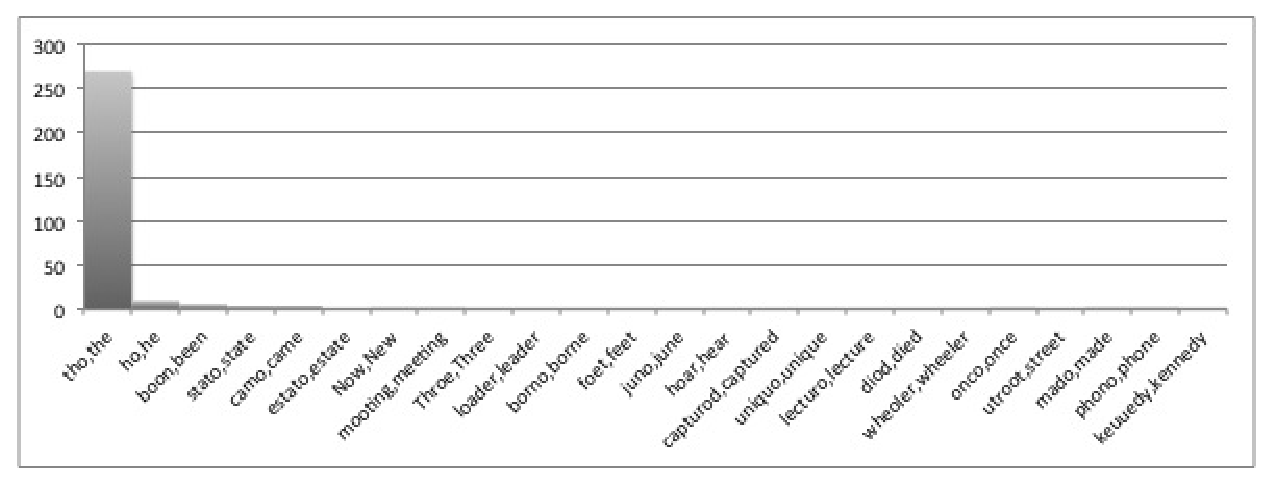
\epsfig{file=o_e.eps, height= 2.2 in,width= 5.5 in}
\caption{Examples of o $\rightarrow$ e corrections, (tho,the; ho,he; boon,been; stato,state; camo,came; estato,estate; Now,New; mooting,meeting; throe,three; loader,leader; borno,borne, foet,feet; juno,june; hoar,hear; capturod,captured; uniquo,unique; lecturo,lecture; diod,died; wheoler,wheeler; onco,once; utroot,street; mado,made; phono,phone)}
\label{fig:fig3}
\end{figure*}

\begin{figure*}[ht]
\centering
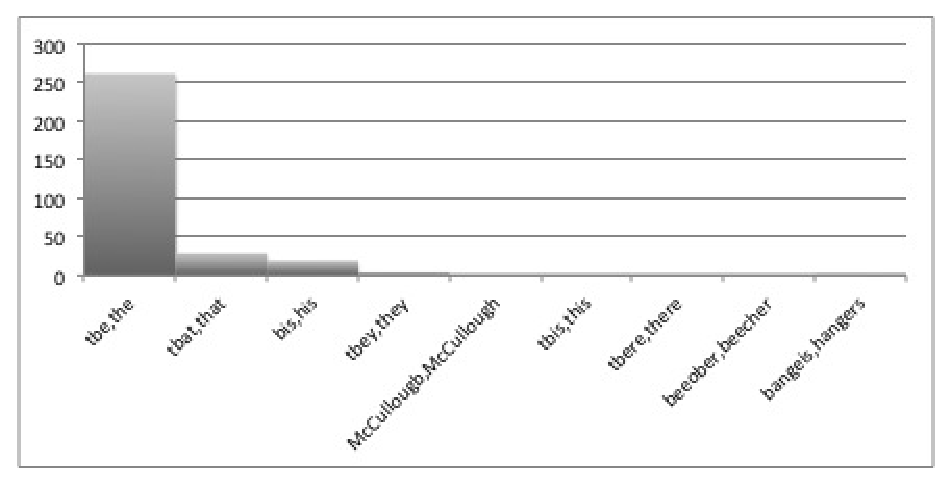
\epsfig{file=b_h.eps, height= 2 in,width= 5.2 in}
\caption{Examples of b $\rightarrow$ h corrections, (tbe,the; tbat,that; bis,his; tbey,they; McCullougb,McCullough; tbis,this; tbere,there; beeober,beecher; banger,hanger)}
\label{fig:fig4}
\end{figure*}

\begin{figure*}[ht]
\centering
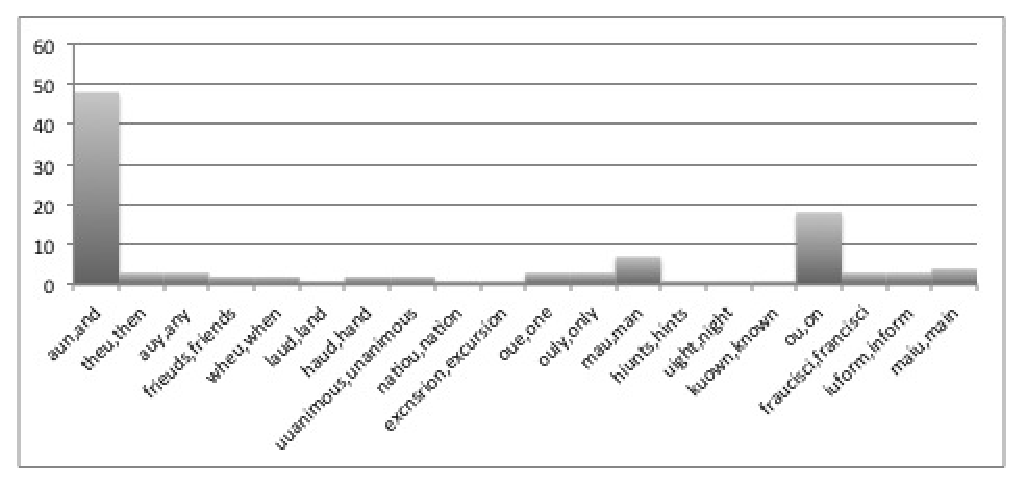
\epsfig{file=u_n.eps, height= 2 in,width= 5.2 in}
\caption{Examples of u $\rightarrow$ n corrections, (aud,and; theu,then; auy,any; frieuds,friends; wheu,when; laud,land; haud,hand; uunanimous,unanimous; natiou,nation; oue,one; ouly,only; mau,man; hiuts,hints; uight,night; kuown,known; ou,on; fraucisci,francisci; iuform,inform; maiu,main)}
\label{fig:fig5}
\end{figure*}

\begin{figure*}[ht]
\centering
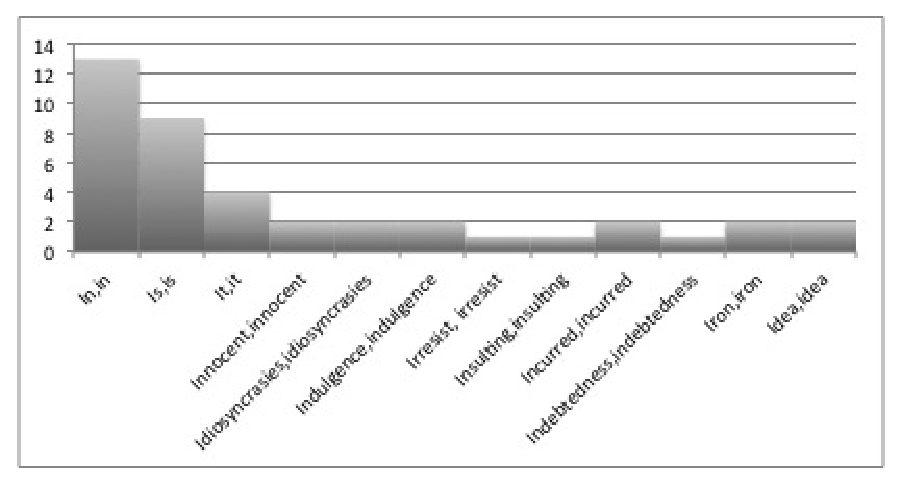
\epsfig{file=I_i.eps, height= 2 in,width= 5.2 in}
\caption{Examples of I $\rightarrow$ i corrections, (In,in; Is,is; It,it; Innocent,innocent; Idiosyncrasies,idiosyncrasies; Indulgence,indulgence; Irresist, irresist; Insulting,insulting, Incurred,incurred; Indebtedness,indebtedness; Iron,iron; Idea,idea)}
\label{fig:fig6}
\end{figure*}

\begin{figure*}[ht]
\centering
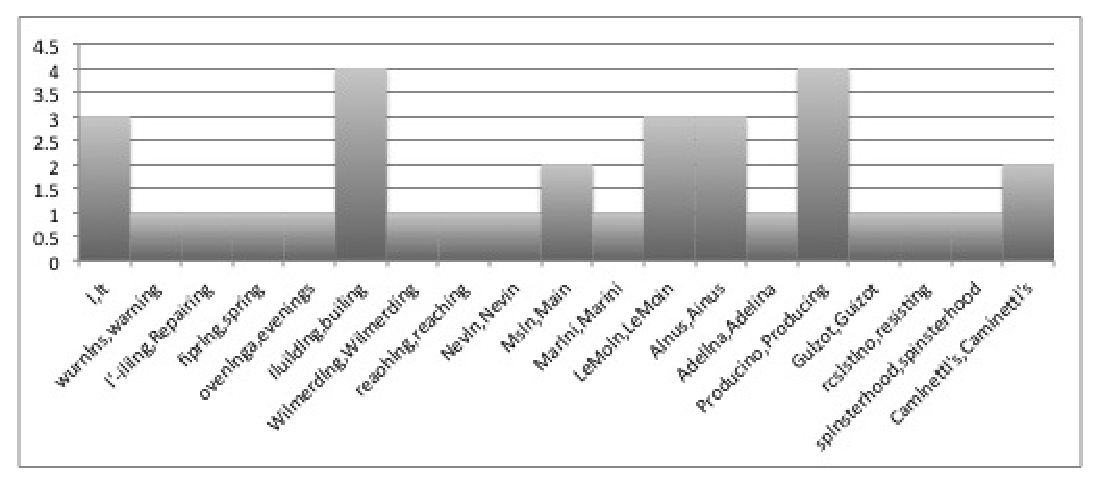
\epsfig{file=l_i.eps, height= 2 in,width= 5.2 in}
\caption{Examples of l $\rightarrow$ i corrections, (l,It; wurnlns,warning; l'-ililng,Repairing; fiprlng,spring; ovenlnga,evenings; Iluildlng,builing; Wilmerdlng,Wilmerding; reaohlng,reaching; Nevln,Nevin; Msln,Main; Marlni,Marini; LeMoln,LeMoin; Alnus,Ainus; Adellna,Adelina; Gulzot,Guizot; rcslstino,resisting; splnsterhood,spinsterhood; Camlnettl,Caminetti)}
\label{fig:fig7}
\end{figure*}


%The rules about hierarchical headings discussed above for
%the body of the article are different in the appendices.
%In the \textbf{appendix} environment, the command
%\textbf{section} is used to
%indicate the start of each Appendix, with alphabetic order
%designation (i.e. the first is A, the second B, etc.) and
%a title (if you include one).  So, if you need
%hierarchical structure
%\textit{within} an Appendix, start with \textbf{subsection} as the
%highest level. Here is an outline of the body of this
%document in Appendix-appropriate form:
%\subsection{Introduction}
%\subsection{The Body of the Paper}
%\subsubsection{Type Changes and  Special Characters}
%\subsubsection{Math Equations}
%\paragraph{Inline (In-text) Equations}
%\paragraph{Display Equations}
%\subsubsection{Citations}
%\subsubsection{Tables}
%\subsubsection{Figures}
%\subsubsection{Theorem-like Constructs}
%\subsubsection*{A Caveat for the \TeX\ Expert}
%\subsection{Conclusions}
%\subsection{Acknowledgments}
%\subsection{Additional Authors}
%This section is inserted by \LaTeX; you do not insert it.
%You just add the names and information in the
%\texttt{{\char'134}additionalauthors} command at the start
%of the document.
%\subsection{References}
%Generated by bibtex from your ~.bib file.  Run latex,
%then bibtex, then latex twice (to resolve references)
%to create the ~.bbl file.  Insert that ~.bbl file into
%the .tex source file and comment out
%the command \texttt{{\char'134}thebibliography}.
%% This next section command marks the start of
%% Appendix B, and does not continue the present hierarchy
%\section{More Help for the Hardy}
%The sig-alternate.cls file itself is chock-full of succinct
%and helpful comments.  If you consider yourself a moderately
%experienced to expert user of \LaTeX, you may find reading
%it useful but please remember not to change it.
%\balancecolumns % GM June 2007
% That's all folks!
\end{document}
